\documentclass[sigconf]{acmart}

\usepackage{booktabs} % For formal tables
\usepackage{lmodern}
\usepackage[T1]{fontenc}
\usepackage[utf8]{inputenc}
\usepackage{float}
\usepackage{subfigure}
\usepackage{amsmath}
\usepackage[textsize=tiny,textwidth=2cm]{todonotes}
\usepackage[ruled,vlined,linesnumbered]{algorithm2e}
\newcommand\mycommfont[1]{\footnotesize\ttfamily\textcolor{black}{#1}}
\SetCommentSty{mycommfont}
\usepackage{algpseudocode}
\usepackage{tikz}
\usetikzlibrary{shapes,arrows,positioning,calc}
\usepackage{url}
\usepackage{pifont}
\usepackage{soul}
\usepackage{pxfonts}
\usepackage{listings}
%\usepackage[hyphens]{url}
\lstset{
backgroundcolor=\color[rgb]{1,1,1},
  basicstyle=\scriptsize,
  columns=fullflexible,
  showstringspaces=false,
  commentstyle=\color{gray}\upshape,
  breaklines=true,
  %frame=single
  keywordstyle=\color{blue},
  numbers=left,
  xleftmargin=5.0ex,
  numberstyle=\tiny\ttfamily\color{black}
}

\lstdefinelanguage{XML}{
  morestring=[b][\color{brown}]",
%  morestring=[s][\color{red}\bfseries]{>}{<},
%  morecomment=[s]{<?}{?>},
  stringstyle=\color{black},
  identifierstyle=\color{blue},
  keywordstyle=\color{cyan},
  escapechar=!,
  morekeywords={name,use,xmlns,version,type}% list your attributes here,
}

\newcommand\encircle[1]{%
  \tikz[baseline=(X.base)] 
    \node (X) [draw, shape=circle, inner sep=0] {\strut #1};}
% Copyright
%\setcopyright{none}
%\setcopyright{acmcopyright}
%\setcopyright{acmlicensed}
\setcopyright{rightsretained}
%\setcopyright{usgov}
%\setcopyright{usgovmixed}
%\setcopyright{cagov}
%\setcopyright{cagovmixed}


% DOI
%\acmDOI{10.475/123_4}

% ISBN
%\acmISBN{123-4567-24-567/08/06}

%Conference
%\acmConference[WOODSTOCK'97]{ACM Woodstock conference}{July 1997}{El
%  Paso, Texas USA} 
%\acmYear{1997}
%\copyrightyear{2016}
%
%\acmPrice{15.00}


\begin{document}
\title{GPaaScaler : Towards Green Energy Aware Scalable Cloud Platform}
%\titlenote{Produces the permission block, and
%  copyright information}
%\subtitle{Extended Abstract}
%\subtitlenote{The full version of the author's guide is available as
%  \texttt{acmart.pdf} document}


\author{MD Sabbir Hasan}
%\authornote{Dr.~Trovato insisted his name be first.}
\orcid{1234-5678-9012}
\affiliation{%
  \institution{INRIA}
  \streetaddress{}
  \city{Nantes} 
  \state{France} 
  \postcode{77}
}
\email{sabbir.hasan@inria.fr}

\author{Frederico Alvares}
%\authornote{The secretary disavows any knowledge of this author's actions.}
\affiliation{%
  \institution{IMT Atlantique}
  \streetaddress{}
  \city{Nantes} 
  \state{France} 
  \postcode{}
}
\email{frederico.alvares@inria.fr}

\author{Thomas Ledoux}
%\authornote{This author is the
%  one who did all the really hard work.}
\affiliation{%
  \institution{IMT Atlantique}
  \streetaddress{}
  \city{Nantes} 
  \country{France}
  }
\email{thomas.ledoux@inria.fr}



% The default list of authors is too long for headers}
%\renewcommand{\shortauthors}{B. Trovato et al.}


\begin{abstract}
This chapter is an ongoing investigation on how to efficiently utilize the elasticity nature of the infrastructure resources when overall resource requirement of an application is higher than the existing underlying infrastructure can handle. Actions like adding/removing resource can be done independently at the infrastructure layer based on their utilization level \emph{i.e.,} cpu usage, memory usage etc. But, every application performs differently from one another at same cpu utilization level, specially when the resource utilization is medium to high. Therefore, coordinating the decision based on applications resource requirement or performance is the better way to devise scaling strategies. To this, firstly we propose to listen events from application to understand when to trigger scaling decision based on reactive and pro-active scaling rules. Secondly, we use traditional API such as \emph{scale-in} and \emph{scale-out} to trigger decision based on the strategy we have devised. Later we want to validate our approach by extensive experiments and results obtained over Grid'5000 test bed. \textcolor{red}{****Rewrite Abstract*****}
\end{abstract}

%
% The code below should be generated by the tool at
% http://dl.acm.org/ccs.cfm
% Please copy and paste the code instead of the example below. 
%
\begin{CCSXML}
<ccs2012>
 <concept>
  <concept_id>10010520.10010553.10010562</concept_id>
  <concept_desc>Computer systems organization~Embedded systems</concept_desc>
  <concept_significance>500</concept_significance>
 </concept>
 <concept>
  <concept_id>10010520.10010575.10010755</concept_id>
  <concept_desc>Computer systems organization~Redundancy</concept_desc>
  <concept_significance>300</concept_significance>
 </concept>
 <concept>
  <concept_id>10010520.10010553.10010554</concept_id>
  <concept_desc>Computer systems organization~Robotics</concept_desc>
  <concept_significance>100</concept_significance>
 </concept>
 <concept>
  <concept_id>10003033.10003083.10003095</concept_id>
  <concept_desc>Networks~Network reliability</concept_desc>
  <concept_significance>100</concept_significance>
 </concept>
</ccs2012>  
\end{CCSXML}

\ccsdesc[500]{Computer systems organization~Embedded systems}
\ccsdesc[300]{Computer systems organization~Redundancy}
\ccsdesc{Computer systems organization~Robotics}
\ccsdesc[100]{Networks~Network reliability}


\keywords{ACM proceedings, \LaTeX, text tagging}

%\acmBadgeR{artifacts_available}

\maketitle
%\title{GPaaScaler : Towards Green Energy Aware Scalable Cloud Platform}

\section{introduction}


The fast growth of internet technology and proliferation of Cloud services have multiplied data centers number in recent years. In 2016, data centers around the world consumed 416.2 TWh of electricity, which is significantly higher than the UK's total consumption of about 300 TWh on the same year\footnote{\url{http://www.independent.co.uk/environment/global-warming-data-centres-to \\-consume-three-times-as-much-energy-in-next-decade-experts-warn-a6830086.html}}. Although, numerous state-of-the-art energy efficient techniques have been adopted by industry and academia, a recent report suggests that energy usage in data centers is expected to increase by 4\% until 2020, which will translate to higher carbon emission. Most of today's data centers consume grid tied brown energy, very few are partially powered by renewable energy. Therefore, energy efficient techniques alone is not going to reduce the
carbon footprint since energy consumption will continue to grow.
On the other hand, the ever increasing enthusiasm and consciousness of reducing energy consumption can lead towards smarter ways to consume energy in cloud data centers. While an efficient energy management technique in data center can reduce unnecessary use of brown energy and better utilize green energy without going to waste \cite{parasol}, \cite{sabbir}, smarter ways of consuming energy in the presence/absence of renewable/green energy by an application can further reduce carbon footprint.

 

Traditionally, data centers host heterogeneous applications, such as \emph{interactive} and \emph{batch} applications/jobs. Goiri et al. \cite{GreenSlot}, \cite{GreenHadoop} first proposed a green energy adaptive framework for batch job oriented tasks \emph{i.e.,} that facilitated the scheduling of these tasks to different times by respecting the deadline when green energy is available. On the contrary, interactive
applications possess lesser flexibility, i.e., it should react with
little to no latency, otherwise Quality of Service (QoS) can
be seriously impacted. To cope up with these limitations, we have proposed a green energy adaptive solution to create green energy awareness inside the application that inherits the capability to smartly use the available green energy having \emph{static} amount of underlying resources \cite{cloudcom},\cite{tsc}.

But in a realistic cloud environment, resource requirement might exceed the currently provisioned resources. In contrast, when fewer resources are required, de-provisioning of resources can help to reduce unnecessary energy consumption. Therefore, the capability to detect when resources are required/dispensable and react to it so as to keep performance at a targeted level while energy consumption can be minimized is required. Taking application reconfiguration decision in isolation with resource scaling policies may lead to performance degradation and inconsistency to the system. Hence, coordination between two different types of elasticity (\emph{i.e.,} application reconfiguration vs infrastructure (de)provisioning) is necessary.

Most of the work in the literature propose: (i) multiple autonomic loops in a coordinated manner to control cluster level resources (\emph{i.e.,} one loop for controlling DVFS, another loop for deciding scaling actions)\cite{server-cluster}, \cite{shi}; (ii) per-application local manager which requests to a central autonomic manager to tune the number of cpu core, memory and to change the number of VM's \cite{morin1}, \cite{morin2}; (iii) adaptive framework to coordinate between system level (DVFS) and application level (degrading quality) adaptation to improve performance and power efficiency \cite{adaptcap}.

It is clearly visible that - synergy between application and infrastructure based on green energy availability is missing despite having elasticity capability in both layers. We believe that, integrating the autonomic logics of the infrastructure with the one in the applications is a important research direction.
Therefore, in response to the existing works, we propose a PaaS (Platform-as-a-Service) solution, named \emph{GPaaScaler} that inherits the capability to adapt both at \emph{application} and at \emph{infrastructure} level in facing to changing condition \emph{i.e.,} workload burst, performance degradation, quality of energy etc. We refer green energy to be better in quality, compared to brown energy.
Application adaptation is realized by dynamically re-configuring application's mode/service level on the fly based on performance and/or green energy availability, whereas infrastructure adaptation takes care of addition/removal of resources based on application's resource demand. During application adaptation, any dynamic change at the software layer that impacts the energy profile can be considered as switching to higher or lower modes/service levels.
To this point, we want to study the impact of application adaptation (based on the presence/absence of green energy) on infrastructure to have a global view of energy consumption incurred by the application.
Furthermore, both adaptation technique is built in separate modules and coordinated in a sequential manner. For example, when application's performance decreases due to heavy load, the PaaS solution first triggers adaptation to application by downgrading the functionality according to signed SLA (Service Level Agreement) and invokes resource requests to infrastructure module. Followed by the invocation requests, infrastructure adaptation module analyzes and decides whether resources are going to be added or the request is to be ignored. We have tested our proposal at Grid'5000 test bed with a real life application, workload and energy profile to show that, when green energy aware adaptation is adopted, around 35\% brown energy consumption can be reduced compared to a baseline approach. By reducing brown energy consumption, ratio of green energy to brown energy can be increased and subsequently carbon footprint can be appreciably reduced.
The rest of the paper is organized as follows. Section 2 describes the GPaaScaler architecture. In Section 3, several Application controllers and a generic Infrastructure controller are designed to investigate their impacts on energy consumption and QoS properties and Section 4 validate approach through extensive experiments. Furthermore, in Section 5, we provide discussion based on results and observation. Section 6 describes the related works and we conclude our work in Section 7.
\section{GPaaScaler architecture}

This section presents our auto-scaler architecture named \emph{GPaaScaler}, which continuously listens the instances of events \emph{e.g.,} response time, green energy availability, working modes of application etc., pushed by SaaS and IaaS in a changing environment. Furthermore, it inherits the capability to actuate both at application and at infrastructure level.
We use the most popular self-adaptive design framework: Monitor-Analyze-Plan-
Execute-Knowledge (MAPE-K) loop \cite{vision} for our auto-scaler.
Our contribution lies on the \emph{analyze} and \emph{plan} (A-P) block of this autonomic framework.

\begin{figure} [ht]
\centering
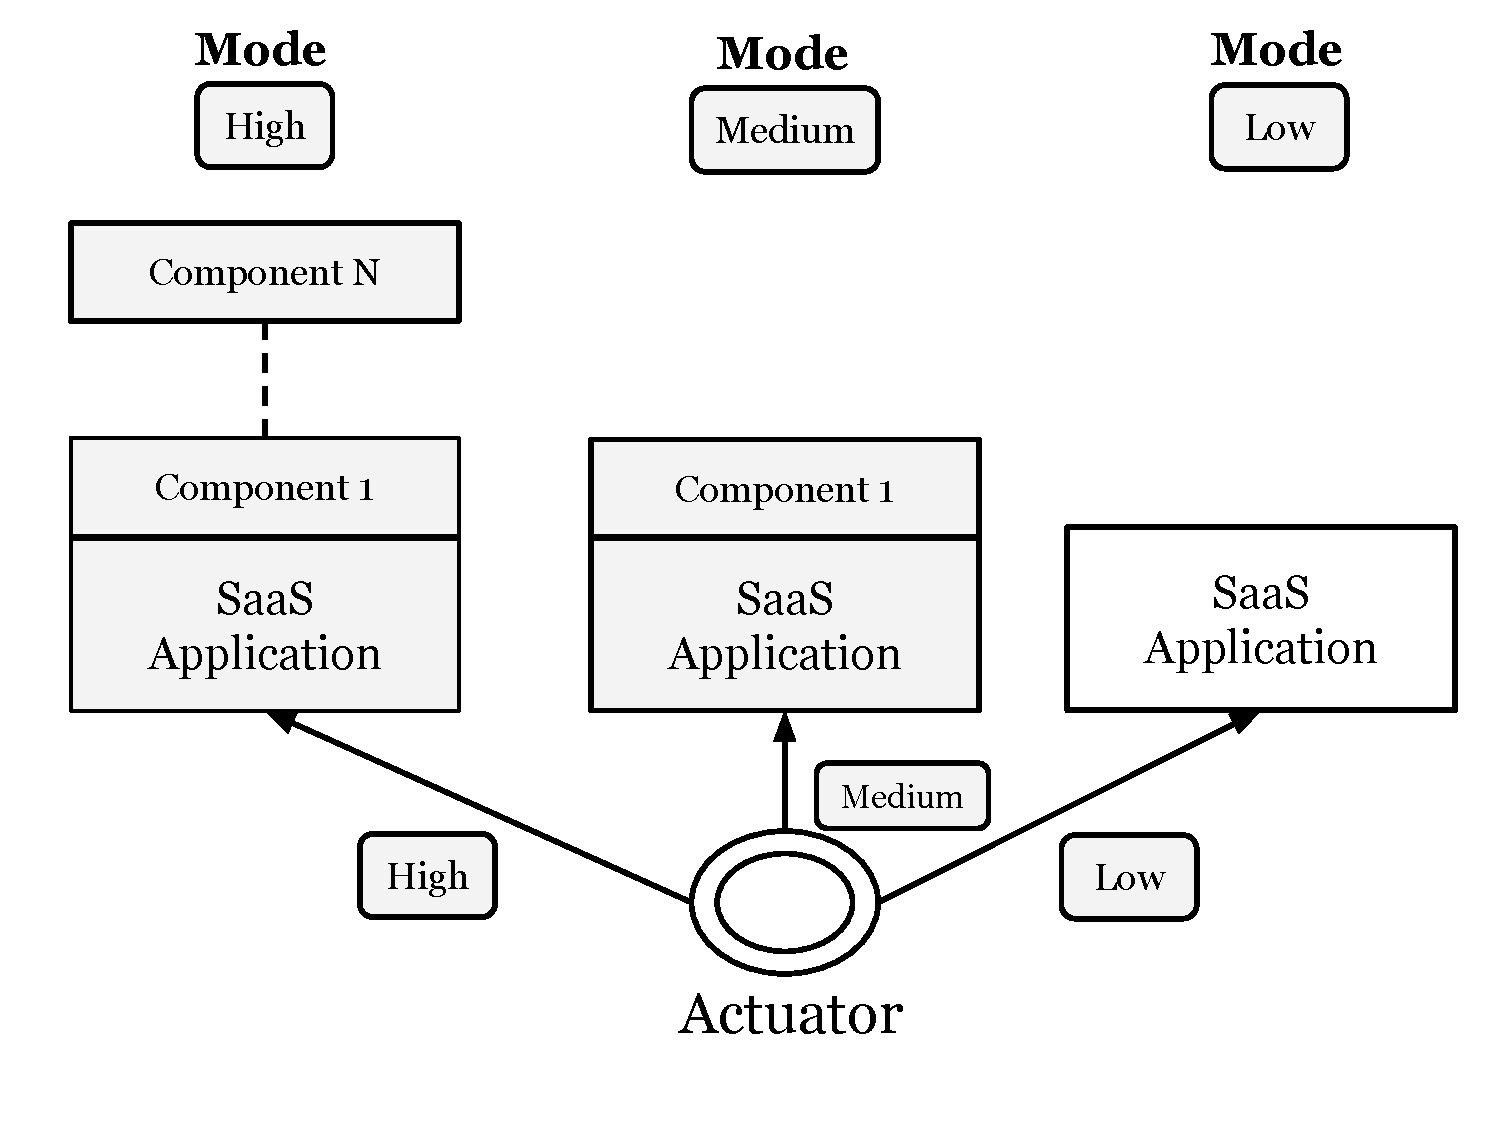
\includegraphics[scale=.32]{Graphs/action_1.pdf}
\caption{Applications mode under different service level}
\label{fig:modes}
\end{figure}

Monitoring (M) block pushes listened events to \emph{Analyze} block from SaaS layer (\emph{i.e.,} response time, workload, application's working mode, etc.) and IaaS layer (\emph{i.e.,} quality of energy). Analyze (A) block is responsible for analyzing and decoupling events to extract the pertinent information and feed appropriate event to the event handler at the SaaS controller. Once the configuration plan is ready, SaaS controller triggers action through SaaS actuator.
We propose three user experience levels. Mode High refers to high user
experience while Mode Medium and Mode Low indicate to medium and low user experience respectively (see Figure \ref{fig:modes}). When current application behavior deviates from target system state in terms of objective metrics, the auto-scaler gracefully downgrades the user experience from higher mode to lower mode and vice-versa through proper actuator value. Once SaaS actuator trigger the adaptation plan, it passes request for addition/removal of resources event as «RequestEvent» to IaaS controller if the former controller decides that application needs more/less resources, which is shown at Figure \ref{fig:GPaaScaler}. Following the event, IaaS controller decides to take action via traditional infrastructure API that is \emph{scale-in} and \emph{scale-out} or wait/discard the request issued by the SaaS controller. Therefore, the execution block is composed of two types of actuators, \emph{i.e.,} SaaS and IaaS actuator, which can be seen at Figure \ref{fig:GPaaScaler}. In addition, \encircle{1}, \encircle{2} and \encircle{3} depict the task flow of our auto-scaler, 
whereas, the sequential flow in an ordered way (from $1.a$ to $1.e$) is presented at the Figure \ref{fig:GPaaScaler} for highlighting the control flow of the event.
In summary, IaaS controller only gets activated if SaaS controller issues any «RequestEvent». However, our proposed IaaS controller are unware of resource allocation strategy, for instance, what types of VM is to be added/removed or in which server VM is to be located etc.  




\begin{figure} [ht]
\centering
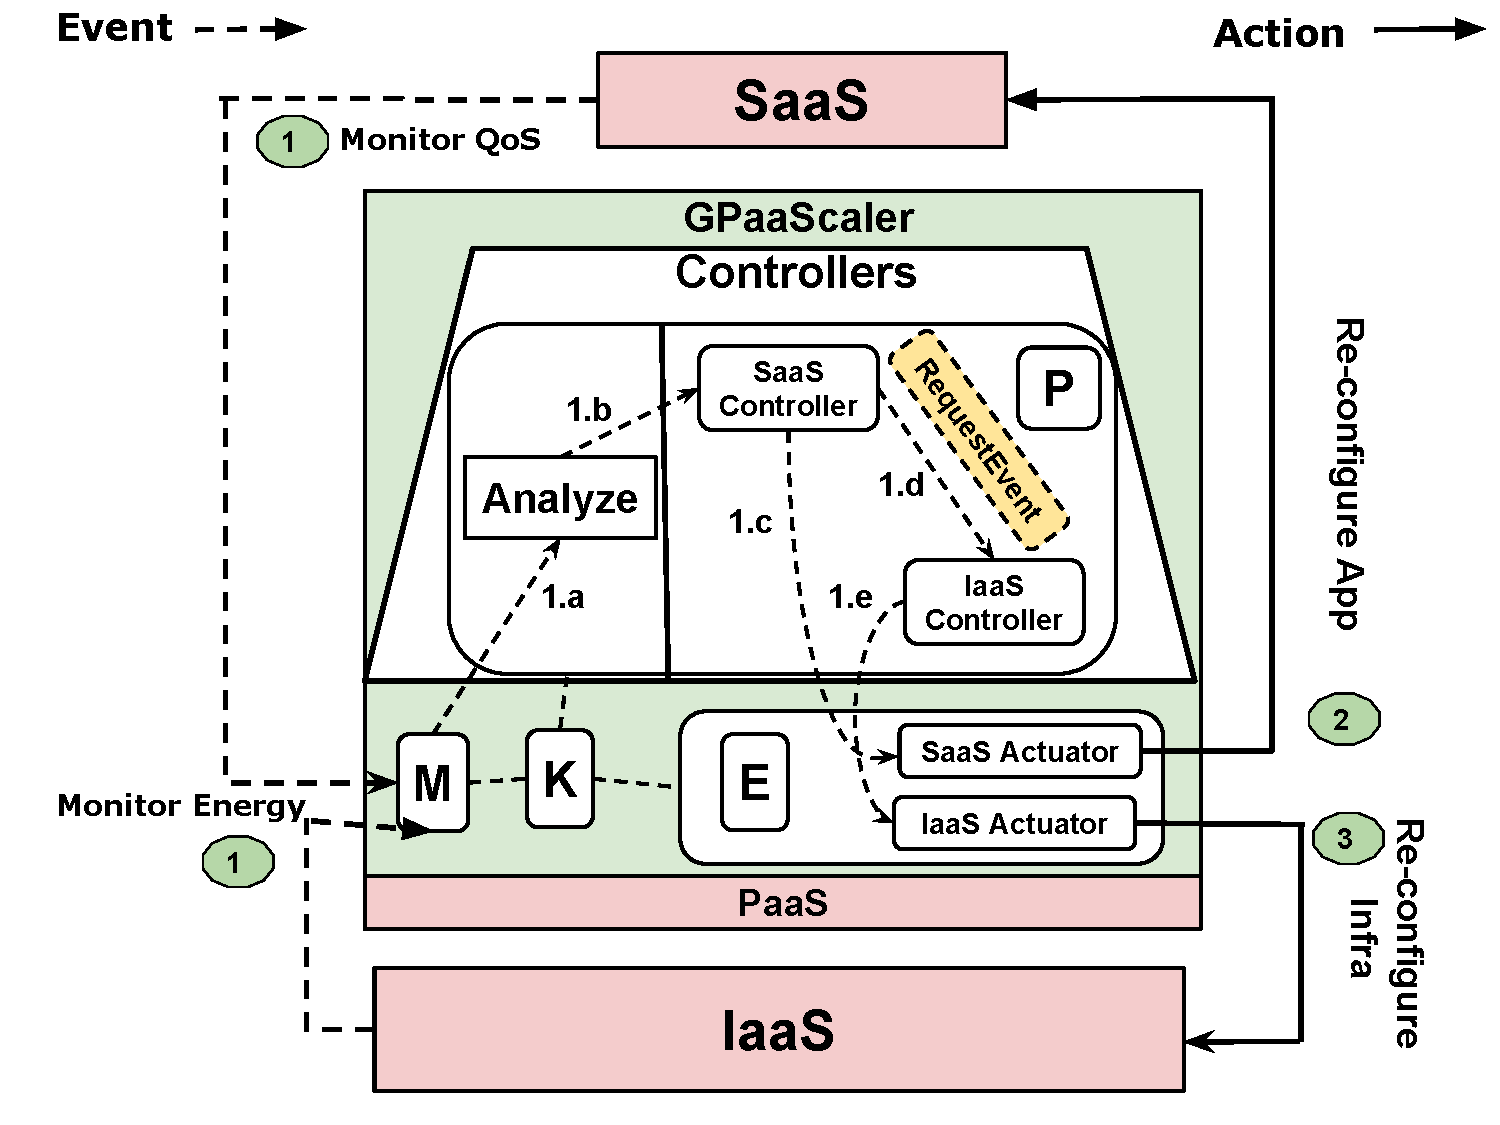
\includegraphics[scale=.38]{Graphs/test_gpaascaler.pdf}
\caption{GPaaScaler architecture}
\label{fig:GPaaScaler}
\end{figure}



\section{Proposed Controllers}

This section describes several application controllers which have been extended to leverage the underlying elastic infrastructure and a generic infrastructure controller which can be plugged with any application controller to control the elasticity capability of cloud infrastructure. 

\subsection{Application/SaaS controllers} \label{saas-controller}

% last chapter presents couple of controller. We choose the most performant one, and most energy efficient one with non-adaptive approach.

We have designed and validated several single and mutiple metric application controllers which have the capability to re-configure SaaS application to keep it accessible and performant even at changing conditions at \cite{sabbir},\cite{tsc}. In this article, we extend the Response time controller (performance aware) and Green Energy Controller (quality of resource aware) with increased capability to request of addition/removal of resources from the underlying elastic infrastructure.


\paragraph*{\textbf{Response Time controller (RT-C)}}
Response time is an essential metric to guarantee cloud
based application's performance. Our goal is to keep response
time under certain threshold dynamically to maximize the
availability of the service in unpredictable and variable
workload condition. We closed the managed software
system by a feedback loop, where in each control period, the
output is forwarded as a Map of response time and workload
arrival rate to compare with the target set-point. Afterwards, the information is forwarded to compute a function:

\begin{equation}
f(t)=1-\tilde{\lambda}(t)*\tilde{r}(t)
\end{equation} 

where \begin{math}\tilde{\lambda}(t) = \frac {\lambda(t-1)}
	{\lambda_{median}}\end{math} and \begin{math}\tilde{r}(t) =\frac
	{RT_{95}(t-1)} {RT_{setpoint}}\end{math}. Since,
unpredictability and burstiness of user requests is common phenomena for Cloud application, we have considered workload arrival rate $\lambda(t)$ as a disturbance to the system. Ignoring the disturbance can lead to dramatic degradation of application performance. For capturing the change in the workload
arrival rate, current workload arrival rate in the system is divided by median of
previous arrival rates. A median filter is used with window size of four, that provides better estimation about variability of the workload arrival rate. 
Furthermore, the function $f(t)$ is computed at each $t$ time to analyze how far the multiplication ratio of workload change and response time increment/decrement is from $1$. The idea is to keep the function greater than $0$ to stabilize
the system to operate under target response time. If the function is positive and above a desired/predefined threshold, the controller keeps the highest user experience mode \emph{i.e.,} mode 2. Since the controller is not aware of how much amount of underlying resources are used, it notifies the \emph{vmRemove} event to the IaaS controller (see line 13, Algorithm \ref{algo:rt_extended}). In case, the condition block falls to \emph{f(t) $\leq 0$}, a «RequestEvent» of \emph{vmAdd} is notified to IaaS controller (see line 10, Algorithm \ref{algo:rt_extended}).





%------------------------------Algorithm 2-------------------------
\begin{algorithm} [!ht]
\DontPrintSemicolon
\footnotesize
\KwIn { $Thr_{rt}, \lambda=[0 \quad 0 \quad 0 \quad 0], setPoint, app$ 
} 
\KwOut { updated $\lambda$, $Curr_{mode}$ = Current application mode. } 

\BlankLine 

\If {($handleEvent == responseTime$)}
     {    $\lambda(t-1)\gets servedRequest \ $ \;
         $enqueue(\lambda)$ \;
         $f(t)\gets 1-(\lambda(t-1)/\lambda_{median})*(RT_{95}/setPoint)$
	  
	   
		\If  { $(f(t) > 0) \enspace\land\enspace\  (function < Thr_{rt})$ } 
			     { $app.mode\gets mode \ 1$\;
			     $RequestEvent \rightarrow vmAdd$ \tcc*[f]{VM \emph{Addition} request event sent to IaaS controller along with $RT_{95}$ and workload-increment = $(\lambda(t-1)/\lambda_{median})$} \;}
		\ElseIf { $f(t) \leq 0$ } 
			{ $app.mode\gets mode \ 0$ \;
			$RequestEvent \rightarrow vmAdd$ \tcc*[f]{VM \emph{Addition} request event sent to IaaS controller along with $RT_{95}$ and workload-increment = $(\lambda(t-1)/\lambda_{median})$} \;}
 			\Else {$app.mode\gets mode \ 2$ \; 
 			       $RequestEvent \rightarrow vmRemove$ \tcc*[f]{VM \emph{Removal} request event sent to IaaS controller along with $RT_{95}$ and workload-increment = $(\lambda(t-1)/\lambda_{median})$} \;}
                $dequeue(\lambda)$ \; 
                $Curr_{mode} = app.mode$ \;			
 			
 			    							 							
 		}
\Return { $\lambda$, $Curr_{mode}$  } 
\caption {Response time controller (RT-C)} 
\label{algo:rt_extended}
\end{algorithm}
%--------------------------%End-%---------------------------------
 



\paragraph*{\textbf{Green Energy Controller (GE-C)}} While \emph{RT-C} is built to avoid performance degradation by keeping
response time to a target set point, is not aware of when green energy production is scarce or abundant to actuate application's mode. On the other hand, devising adaptation plan only based on green energy availability can dissatisfy reasonable QoS while workload arrival is higher.
Therefore, we intend to build a controller which can make adaptive decision based on the better quality of energy \emph{i.e.,} green energy and application's performance. 

We distinguish between two control periods: long and short. Algorithm \ref{algo:h_green_extended} presents two <<handleEvent>> blocks, each associated with specific event \emph{i.e.,} $greenEnergy$ and $responseTime$.
In \emph{longer control period}, $greenEnergy$ block decides application's mode based on green energy availability. Some sources of green energy are only available during certain times. For instance, solar energy is available during the day and the amount produced depends on the weather and the season \cite{GreenHadoop}. Due to the intermittency, we have divided the total green energy production to three different regions \emph{i.e.,} no green energy (at night), few (early morning and late afternoon) and adequate (mid-day). To distinguish between the regions we choose a static threshold $Thr_{max}$, above which the controller activates high user experience mode (mode 2). When green energy production falls between $0$ and $Thr_{max}$, the controller chooses an actuator value that triggers the medium user experience mode (mode 1), and in case of current green energy amount is null, mode 0 is activated. In short, the controller activates higher or lower user experience mode based on the energy information pushed by infrastructure in longer control periods. In contrast, the
$responseTime$ block checks the response time periodically in \emph{shorter control period} to identify overloaded condition in the system. If occurred,
the controller downgrades the user experience to lower level. In summary, depending on the event, the specific block gets activated in Algorithm \ref{algo:h_green_extended}.

Afterwards, we try to investigate when performance indicator of an Application can trigger add/remove VM request. Since this controller have two feedback loops activating at two different control periods: long and short, and longer control period's decision depends only on the energy information, hence we focus on the shorter control period loop which is based on response time event. The shorter control loop periodically checks if the targeted response time is violated by application by computing a function at line 15 at Algorithm \ref{algo:h_green_extended}. If the computed function becomes negative (f(t) $\leq 0$) meaning, if the current response time is beyond or borderline to set point and/or the tendency of the workload is increasing, the controller downgrades the user experience by subtracting 1 from previous control period's decision value and notify a \texttt{vmAdd} event request to the infrastructure controller (see line 18, Algorithm \ref{algo:h_green_extended}). While the function is greater than $0$, which suggests that the application is performing well by keeping current 95th percentile response time to the set point, application keeps the user experience as before but notify a \texttt{vmRemove} event request to the infrastructure controller (see line 21, Algorithm \ref{algo:h_green_extended}). In both cases, «RequestEvent» notifies the specific event along with application's current 95th percentile response time and workload increment ratio to the IaaS controller.

%------------- ALgorithm Green hybrid_extended -------------------------
\begin{algorithm} [!ht]
\DontPrintSemicolon
\footnotesize
\KwIn { $Thr_{max}$ = Threshold for green energy, $\lambda=[0 \quad 0 \quad 0 \quad 0]$, $setPoint$,$Curr_{GE}$ = Current green energy production. } 
\KwOut { updated $\lambda$, $Curr_{mode}$ = Current application mode.  } 

\BlankLine 
\emph{/* Initiates in longer control period */}\;

\If {($handleEvent == greenEnergy$)} 
{
\If  { $Curr_{GE} == 0$ } 
			     { $app.mode\gets mode \ 0$\;}
		\ElseIf { $Curr_{GE}>Thr_{max}$ } 
			{ $app.mode\gets mode \ 2$ \;}
 			\Else {$app.mode\gets mode \ 1$ \;}
 			      $Curr_{mode} = app.mode$ \;  
 			     }
\Return { $Curr_{mode}$ } 			      			   
\BlankLine  
\emph{/* Initiates in shorter control period */}\;  
  \If {($handleEvent == responseTime$)} 
     {    $\lambda(t-1)\gets servedRequest \ $ \;
         $enqueue(\lambda)$ \;
         $f(t) \gets 1-(\lambda(t-1)/\lambda_{median})*(RT_{95}/setPoint)$
	  
 \If { $(f(t) \leq0) \quad and  \quad (Curr_{mode} \neq0)$ }
			     { $app.mode\gets Curr_{mode}-1$ \;
			       $RequestEvent \rightarrow vmAdd$ \tcc*[f]{VM \emph{Addition} request event sent to IaaS controller along with $RT_{95}$ and workload-increment = $(\lambda(t-1)/\lambda_{median})$} \;}
 			\ElseIf {$(f(t)>0)$ }
 			{ $app.mode\gets Curr_{mode}$ \;
 			$RequestEvent \rightarrow vmRemove$ \tcc*[f]{VM \emph{Removal} request event sent to IaaS controller along with $RT_{95}$ and workload-increment = $(\lambda(t-1)/\lambda_{median})$} \;}
           
         \Else { $app.mode\gets Curr_{mode}$ \; }          			
             $Curr_{mode} = app.mode$\;
             $dequeue(\lambda)$ \;        			
           } 
              
\Return { $\lambda$, $Curr_{mode}$ } 
\caption {Green Energy controller (GE-C)}
\label{algo:h_green_extended}
\end{algorithm}






\subsection{IaaS controller}


While under-provisioning of resources can significantly hamper QoS properties by saturating application, over-provisioning of resources can increase energy consumption and other associated costs significantly. Therefore, the scaling decision, for instance, add resources (scale-out) or remove resources (scale-in) should be taken carefully to match with the applications resource demand. To meet \emph{scale-out} condition, a reactive policy can be easily designed and implemented based on the monitored performance metrics or by listening to predefined appropriate events. A reactive policy is referred to a runtime decision based on current demand and system state - to add resources on the fly. On the contrary, reactive policies can not absorb the non-negligible resource/instance initiation time. In our case, when application starts to face high response time, both the SaaS controllers have the capability to downgrade the user experience level and to invoke an implicit event (\texttt{vmAdd}) request to IaaS controller. Therefore, the sequential operation can trigger the application to run at lower mode until the instance is launched and activated. Afterwards, the application reverts back to higher mode if it meets the condition after operation.

In contrast, when \emph{scale-in} event (\emph{i.e.,} fewer resources are required by application) is invoked by SaaS controllers, terminating instance based on reactive policy can have detrimental impact on the system \cite{magali}. For example, when application performs better by staying just below or borderline to set point, triggering \emph{scale-in} action can make an application suffering from high response time to saturation. One way to overcome the problem is to VM resizing, that is to reduce the number of cpu cores on the fly by doing fine-grained analysis of resource requirements rather than terminating an entire instance, but popular hypervisors like KVM, VMware, Hyper-V does not allow removing cpu cores of guest VMs at runtime \cite{vertical}.
Additionally, instance termination can cause a sharp rise in response time reaching beyond the set point if workload's behavior or tendency is not taken into consideration. Therefore, devising a plan when to execute \emph{scale-in} event is critical. On the other hand, if the consecutive scaling actions are carried out too quickly without being able to observe the impact of scaling action to the application, undesirable effects such as over and under-provisioning can occur which can leads to performance degradation and/or wastage of energy consumption.
  
%------------- IaaS controller -------------------------
\begin{algorithm} [!ht]
\DontPrintSemicolon
\footnotesize
\KwIn { $[minVm , maxVm]$ = Minimum and maximum number of VM's. \\
$[RT_{95} , workload_{inc}]$ = Response time and workload increment sent by SaaS controller. \\
$[rt_{thr} , decWorkPerc]$ = Two tunable parameters.}
 
\KwOut { $vmNumber$, $coolingPeriod$ } 

\BlankLine 
%\emph{/* \textcolor{red}{Initiates in longer control period} */}\;

\If {($handleEvent == vmAdd$)} 
{
\If  { $(currentTime \notin coolingPeriod) \enspace \land \enspace(vmNumber < maxVm)$ } 
			     { $triggerAction \rightarrow "scale-out"$ \tcc*[f]{Passing API call through cloud infrastructure manager}\;
			       $vmNumber+=1$ \;
			       $coolingPeriod+=coolingLength$ \;
			       }
		
 			\Else {$vmNumber=this.vmNumber$ \;
 			       $coolingPeriod=this.coolingPeriod$ 
 			       }
 			       $vmNumber = update(vmNumber)$ \;  
 			       $coolingPeriod = update(coolingPeriod)$ \;
 }
 
\Return { $vmNumber$, $coolingPeriod$ } 			      			   
\BlankLine  
  
 \If {($handleEvent == vmRemove$)} 
 {
 \If  { $(currentTime \notin coolingPeriod) \enspace\land\enspace(rt_{thr} > RT_{95}) \enspace \land \enspace (vmNumber > minVm) \enspace \land \enspace ((workload_{inc} < decWorkPerc) \enspace \lor \enspace (Curr_{mode}=0))$ }
     
                   { $triggerAction \rightarrow "scale-in"$ \tcc*[f]{Passing API call through cloud infrastructure manager} \;
			       $vmNumber-=1$ \;
			       $coolingPeriod+=coolingLength$ \;
			       }
	  
                  \Else {$vmNumber=this.vmNumber$ \;
 			       $coolingPeriod=this.coolingPeriod$ \;
 			       }
 			       $vmNumber = update(vmNumber)$ \;  
 			       $coolingPeriod = update(coolingPeriod)$ \;
 }
 
\Return { $vmNumber$, $coolingPeriod$ } 
\caption {Infrastructure controller}
\label{algo:iaas_controller}
\end{algorithm}
%--------------------- END -----------------------------   

Hence, the idea is to built a generic IaaS controller which is characteristically agnostic to SaaS controllers behavior. Whenever, an implicit event invocation (\texttt{vmAdd, vmRemove}) arrives to the controller, it activates the proper module by matching to the event. Since, two non-concurrent events can be invoked by SaaS controllers, our proposed IaaS controller contains two modules to handle each of them. We define a length of period called \emph{coolingLength}, which is composed of instance activation time and the time it requires to impact on the application. Therefore, after triggering any scaling decision, this time period is updated to prevent any scaling decision to be made in between. Hence, when \texttt{vmAdd} event arrives to the controller, the $handleEvent == vmAdd$ module matches the condition of not being at $coolingPeriod$ with an and operator 
to maximum number of VM's a provider can be assigned to\footnote{Amazon EC2 permits maximum 20 on-demand instances per user.}. If it adheres the condition, \emph{scale-out} decision is triggered via IaaS actuator and current number of VM and next $coolingPeriod$ is updated (see line 3-5 of Algorithm \ref{algo:iaas_controller}). Otherwise, the module ignores the notification. On the other hand, when \texttt{vmRemove} event is invoked by SaaS controller, if the $handleEvent == vmRemove$ module is not carefully designed, cloud application can face unstable phases \emph{i.e.,} sharp rises of response time to saturate application. Therefore, only looking at $coolingPeriod$ and minimum number of VM
%\footnote{For a 3-tier application, at least one VM per tier should always run.}
 could be unwise and skeptical. 
 
To overcome this situation, we introduce two key parameters which are tunable to identify when is the good time to release resources \emph{i.e.,} perform scale-in action. The parameters are i) how far the current system's response time should be from set point? For example, x\% less than target response time set point, which is denoted by $rt_{thr}$ at Algorithm \ref{algo:iaas_controller}. ii) how much workload rate should decrease from the current trend? For instance, y\% decrease in user requests than previous intervals, denoted by \emph{decWorkPerc}. Hence, when $handleEvent == vmRemove$ arrives to the IaaS controller, the module checks the cooling period, minimum number of VM, current response time condition
with an AND operator. Additionally we put an OR operator between workload decrease parameter and current mode of the application. The rational behind that, in the absence of green energy, \emph{GE-C} controller keeps the application at minimum level. Although, workload may be consistent or increasing, if this application controller invokes \texttt{vmRemove} event that matches to be outside of $coolingPeriod$, greater than minimum number of VM and reduced response time than the threshold, it will meet the \emph{scale-in} condition and IaaS controller will trigger the action to release resources. On the other hand, \emph{RT-C} will keep application at the highest mode when resources are slightly to abundantly over-provisioned. Thus, application being at $mode=0$ and decreasing workload by y\% percentage can not happen concurrently if response time is x\% less than response time set point for this type of SaaS controller. Apart from \emph{GE-C}, any SaaS controller which invokes \texttt{vmRemove} event and satisfies all the conditions mentioned above other than application mode being at lowest, will trigger \emph{scale-in} action by IaaS controller.



%checks if the notification does not exist in coolingPeriod and if it exceeds the maximum amount of VM or not, if not it triggers scale-out action via IaaS actuator. 

%now dive into controller!
\section{Evaluation}
In this section, we present the evaluation results of proposed SaaS and IaaS controller and their impact on cloud based application
in terms of response time and energy consumption. The goal is to advocate the benefits
and limitations of each controller while experimenting
with real cloud application and real workload traces.

\subsection{Experimental setup}
\paragraph*{\textbf{Infrastructure configuration}}The experiments were conducted in Grid'5000 Lyon site,
with 3 physical machines linked by a 10 Gbit/s Ethernet
switch and connected to wattmeter. Each machine has two
2.3GHz Xeon processors (6 cores per CPU) and 16GB of
RAM, running Linux 2.6. Openstack Liberty was used
as platform, which requires one dedicated physical machine
for the cloud controller management system. Consequently,
the other physical machines were used as compute nodes to
host VMs, which in turn, are pre-configured to run Ubuntu
12.04.

\paragraph*{\textbf{Application Configuration}} We experimented with
RUBiS application \cite{rubis}, an eBay like auction site, which
is assumed to be a representative of popular e-commerce application 
and hence interactive web application. In Brownout \cite{brownout}, authors provided a user-to-user recommendation engine that is not core functionality of service but can enhance user experience. Along with that, we implemented a fairly simple item-to-item recommendation, to offer another level of user experience, which is showed at Listing 1. 

\begin{lstlisting}[language=SQL,caption={SQL statement for the recommender system.}, label={sql}]
SELECT
   items1.id
FROM
   items AS items1.id
   JOIN comments AS c ON items1.id = c.item_id
   JOIN items AS i2 ON items1.category = i2.category
 WHERE 
   i2.id = :current_item_id AND
   items1.nb_of_bids >= i2.item_id AND
   items1.id != :current_item_id
ORDER BY rating DESC
LIMIT 10;   
\end{lstlisting}


The
simple recommendation engine can be summarized as "Retrieve 10 products from same seller and same product category which has higher or same user bid count with high customer rating". Although both the
recommendation engines lack the sophistication and worldly complexities, they do
serve as a reasonable example of providing user experience that a cloud
application can isolate from core functionality of the service 
to activate or
deactivate at runtime. The recommendation is added
to the item visualisation page and to enable it, we defined
a function that reads a file, where actuator value is updated
in each control period and execute the associated modes for
each user request. For instance, Mode 1 activates the codes of
recommendation one, mode 2 activates both recommendations
and mode 0 provides no recommendation. Popular e-commerce providers provide multi-level recommendations to their users. Furthermore, the application is deployed with all its tiers \emph{i.e.,} web and database server inside a VM using a LEMP stack\footnote{\url{https://lemp.io/}}. Each application VM and Load-balancer (LB) VM were configured with 4 cores of CPU and 8GB of memory similar to Large flavor VM. Since, we used 2 compute servers, we could use maximum of 6 VM's and minimum at 2 VM's\footnote{1 LB VM and 1 application VM}. 

\begin{figure}[h]
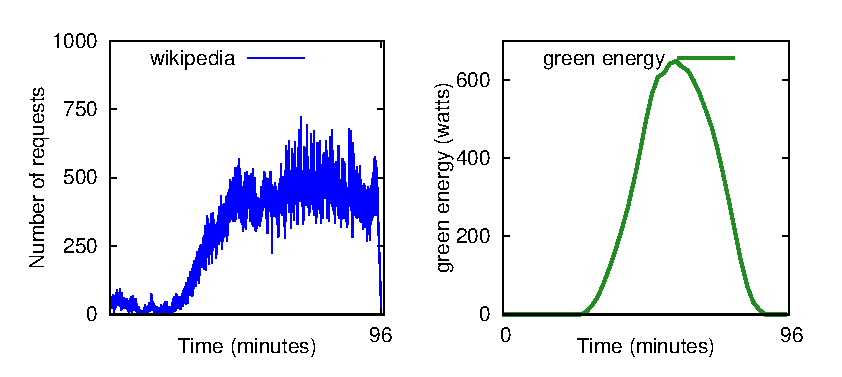
\includegraphics[scale=.7]{Graphs/workload_ucc.eps}
\caption{Workload trace}
\label{fig:workload} 
\end{figure}

\paragraph*{\textbf{Platform and Workload}} Our Proposed platform solution is hosted inside the cloud controller
machine. It monitors the 95th percentile response
time by aggregating the Nginx log of LB in each control period \emph{i.e.,} 20 seconds, whereas green energy
information is pushed by the infrastructure through an API in every 60 seconds. We have set $rt_{thr}$ 80\% and $decWorkPerc$ to 20\% at IaaS controller to evaluate our proposal.
We took the real traffic pattern of wikipedia german page of one day [22] and scaled the data set to fit with our experiment,
which is showed at Figure 6. To generate the workload, we used Gatling as load injector and choose an
open system model, where user requests are issued without
waiting for other users response from the system. Furthermore,
we emulated read-only workload where each user arrives to the homepage, browse any item category from a
vast catalog, click on a product to extract its information,
view seller rating and his/her reputation related to the
product. Furthermore, the duration
of each experiment was 96min and each was run several
times. We considered 96min as 24 hours, i.e., each 4min in
our experiments correspond to 1 hour.


\subsection{Consideration of delaying event}

\begin{figure} [htb]
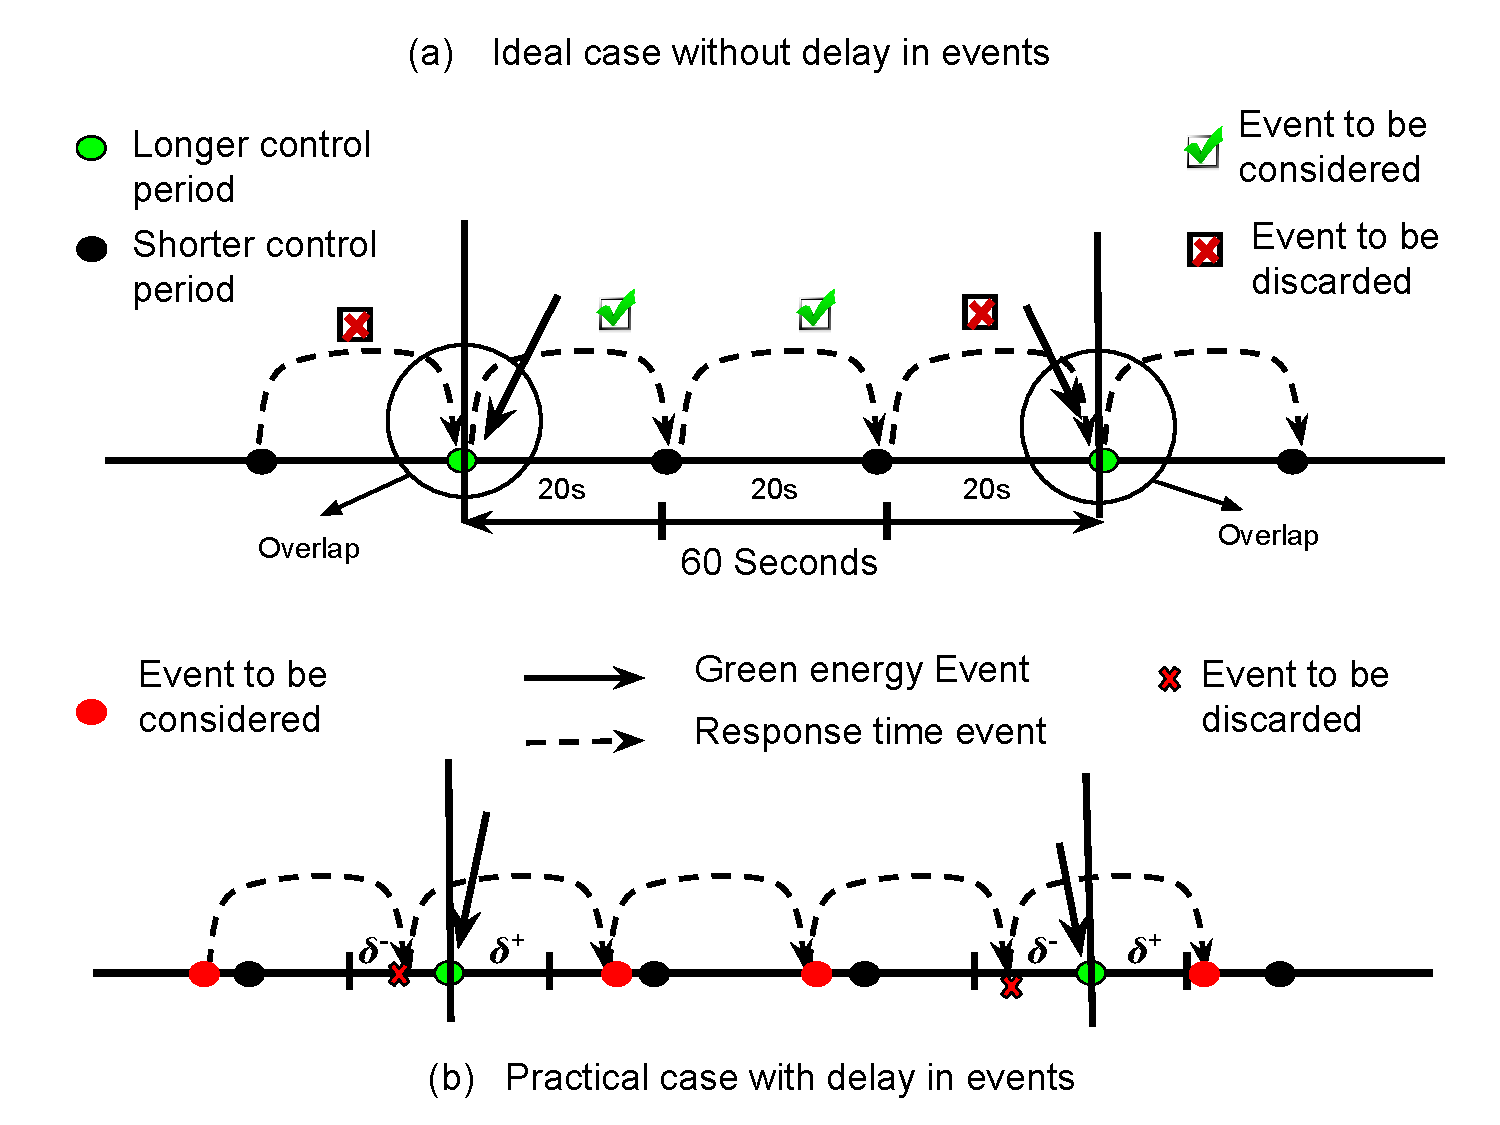
\includegraphics[scale=.35]{Graphs/implementation_UCC.pdf}
\caption{Algorithm implementation in detail}
\label{fig:implementation} 
\end{figure}

From Section \ref{saas-controller}, we see that, \emph{GE-C} controller has inner and outer loops which are activated in different time-scales and push events to the controller to make decision. In our experiments, outer (longer control period) and inner (shorter control period) loops are activated in each 60 seconds and 20 seconds respectively, which is showed in Figure \ref{fig:implementation}. Ideally, if both kind of events arrive without any delay, two different events will overlap each other. As our motivation is to maximize of green energy usage for \emph{GE-C} controller, we always make primary decision based on the green energy event pushed by IaaS by ignoring the response time event which is activated as inner loop, if both the event arrives concurrently. Concretely, it suggests that, between two big decision events in 60 seconds, we consider only two inner loop events and take actions if it is necessary indicated in Figure \ref{fig:implementation}(a).

But in case of delaying of any event, the scenario will not follow Figure \ref{fig:implementation}(a). As discussed before, the primary decision always depends on green energy event. Even though we receive response time event, no action is taken unless the system's response is high. Therefore, in case of delaying of response time event by micro to milliseconds, effects to the system remain almost unchangeable. In contrast, if the event delays by couple of seconds, for instance, inner loop event arrives just before or after the primary decision is made, it might affect the system dynamics to achieve the goal. To tackle the problem, we define a safety distance, denoted by $\delta^t$ to ensure that the controller does not take any action if response time event arrives in between "\textit{PrimaryDecision - $\delta^t$}" and "\textit{PrimaryDecision + $\delta^t$}". Figure \ref{fig:implementation}(b) illustrates the phenomena by an example. For our case, we choose safety distance as, $\delta^t$ = Time frequency of inner loop / $2$, which is equal to 10 seconds in our experiments.



\subsection{Results}

This section elaborately presents the results obtained during experiment at Grid'5000. We consider a baseline approach \emph{i.e.,} non-adaptive controller (NA), which lacks the capability of application adaptation and rely only on infrastructure adaptation based on response time.

%------------------------------------END-------------------------------------

\paragraph*{\textbf{Response time}}
\begin{figure} [htb]
\centering
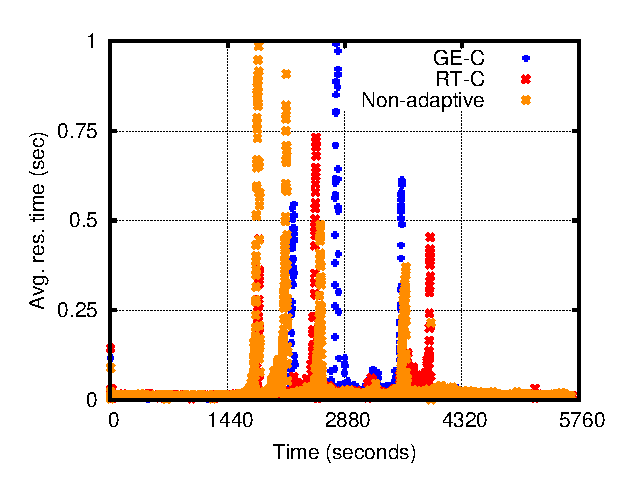
\includegraphics[scale=.8]{Graphs/responseTime.eps}
\caption{Response time incurred by Controllers}
\label{fig:rt}
\end{figure}
In Figure \ref{fig:rt}, we grouped response time by taking average over seconds. We kept response time set point as 1s. Since, our approach allows both level of adaptation depending on the changing environment, both RT-C and GE-C performed very closely by keeping 99th percentile response time around 274ms and 388ms. Figure \ref{fig:perc} shows the distribution of response time. Although, the baseline approach lacked application adaptation, it kept the 99th percentile response time around 500ms. On average, 3.7 million requests were injected during every experiment and only 7-20 requests failed for RT-C and 70-100 requests failed for GE-C. Therefore, both the controller ensure availability to five 9's (99.999\%).

%NA-.473
%GT-C-.388
%Rt-.274

\begin{figure} [htb]
\centering
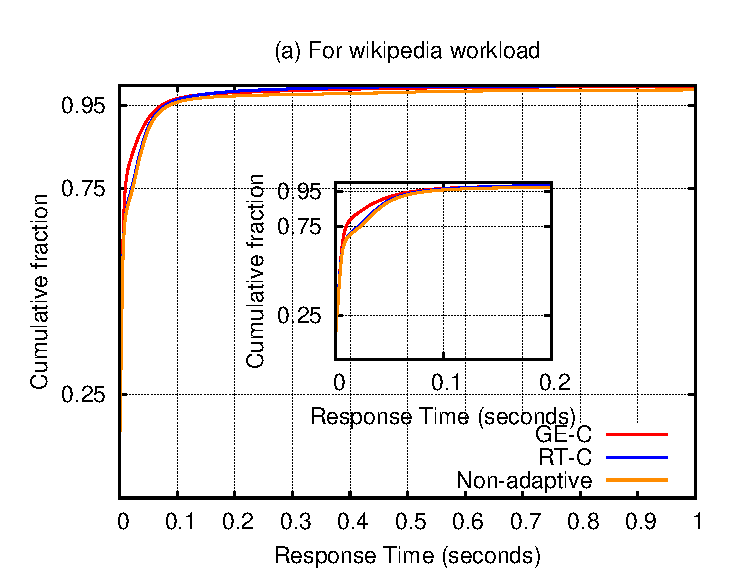
\includegraphics[scale=.75]{Graphs/percentile.eps}
\caption{Response time in percentiles}
\label{fig:perc}
\end{figure}





%----------------------------END-------------------------------------

\paragraph*{\textbf{Energy Consumption}}

In our experiment, each 4 minutes were considered as an
hour, thus we calculated the energy consumption of 24
hours, impacted by each controller, which is presented at
Table \ref{tab:watt1} and \ref{tab:watt2}. Each experiment was run several times and we found the energy consumption difference between each run
was 1$\sim$2 watts. At first, we scaled down the wikipedia workload to test the application controllers with static infrastructure, that is, in any given time application controllers were unable to use underlying elastic infrastructure. Table \ref{tab:watt1} summarizes that, GE-C can reduce brown energy consumption by 9.02\% and 6.4\% compared to NA and RT-C, while total energy consumption was reduced by 6.53\% and 6.4\% respectively. NA was supposed to consume more energy than RT-C since it lacks the capability to adapt application to lower level. Due to the heavy  user requests at some periods, NA approach saturated RUBiS application which was unable to accept any requests which resulted lower availability and lower energy consumption.

%Total: 5912.49
%Green: 3395.9
%Brown: 2516.59

\begin{table*}
\caption{Energy Consumption in Watts (Application adaptation)}
  \label{tab:watt1}
\begin{tabular}{cccl}
\toprule
Controller & Total Energy Consumption & Brown Energy Consumption & Green Energy Consumption\\
\midrule
Non-Adaptive & 3424.20 & 1934.66 & 1484.54 \\
RT-C & 3493.93 & 1975.18 & 1518.75  \\  %&1446.01 & 1941.32 & 3387.33 & --\\ \hline
GE-C & 3270.20 (NA > 6.53\%)(RT-C > 6.4\%) & 1760.09 (NA > 9.02\%) (RT-C > 10.88\%) & 1510.11 (NA < 1.2\%)\textcolor{red}{( RT-C > 0.50\%)} \\
\bottomrule
\end{tabular}
\end{table*}

%Rt & 3493.93 & 1975.18 & 1518.75  \\ \hline %&1446.01 & 1941.32 & 3387.33 & --\\ \hline
%Hybrid-Green & 3270.20 (6.4\%) & 1760.09 (10.88\%) & 1510.11 \alert{(0.50\%)} \\\hline

Afterwards, we proceeded with usual settings with the experiment having infrastructure elasticity capability for all the application controllers. Table \ref{tab:watt2} shows that, GE-C can reduce significant amount of brown energy by 35.11\% and 26.65\% compared to NA approach and RT-C respectively. Interestingly, RT-C consumed less green energy than the other application controllers, although this application controller was designed to consume more green energy than its counterpart application controllers. The reason being that, RT-C activated higher application mode  only in the presence of green energy, irrespective to the amount of user requests. Therefore, if the user requests are lower/higher while few green energy is available the controller activates medium service level mode (\emph{i.e.,} mode 1 which activates 1 kind of recommendation) and starts activating higher service level(\emph{i.e.,} mode 2 which activates 2 different kind of recommendation) when the amount of green energy increases. On the other hand, when green energy is scarce, application works at a low service level mode, that is, user can access the system but no recommendation is provided. In this experiment, the user requests started growing when green energy were scarce. Therefore, NA and RT-C both activated more application VMs than GE-C to cope up with the workload, which can be seen at Figure \ref{fig:vm}. Moreover, Figure \ref{fig:vm} shows that, GE-C followed green energy profile very closely while activating application Vms. It was possible due to fact that, we created green energy awareness to the application through \emph{GPaaScaler}. GE-C and RT-C both used maximum of 4 VM's while NA approach used 5 VM's for same workload.



\begin{table*}
\caption{Energy Consumption in Watts (Application and Infrastructure adaptation)}
  \label{tab:watt2}
\begin{tabular}{cccl}
\toprule
Controller & Total Energy Consumption & Brown Energy Consumption & Green Energy Consumption\\
\midrule
Non-Adaptive & 5912.49 & 2516.59 & 3395.9 \\
RT-C & 5574.78 & 2226.16 & 3348.62  \\  %&1446.01 & 1941.32 & 3387.33 & --\\ \hline
GE-C & 4796.17 (NA > 18.88\%)(RT-C > 13.96\%) & 1632.77 (NA > 35.11\%) (RT-C > 26.65\%) & 3163.4 \textcolor{red}{(NA > 6.83\%)( RT-C > 5.53\%)} \\
\bottomrule
\end{tabular}
\end{table*}

\begin{figure} [htb]
\centering
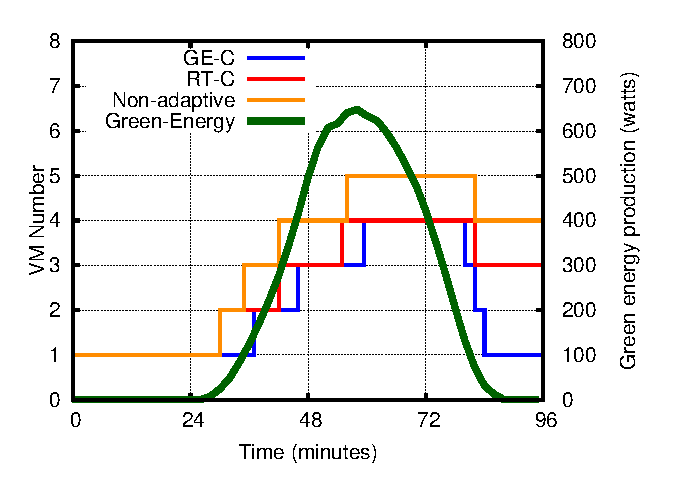
\includegraphics[scale=.8]{Graphs/vm.eps}
\caption{Number of VM usage during experiment}
\label{fig:vm}
\end{figure}

%----------------------------------END-------------------------------------

%0 Non-adaptive 8.748
%1 RT-C 6.696 (23.45 %)
%2 GE-C 5.508 (37.03 %) (21.568 %)

\paragraph{\textbf{Cost analysis}}

Since, our proposed GPaaScaler architecture is agnostic to infrastructure provider and type, it can be plugged on top of public cloud infrastructure. Therefore, we wanted to validate how much each application controller would cost with same application and workload profile. Since, we used large flavor VM's, we fixed instance costs to 0.104 \textdollar

\begin{figure} [htb]
\centering
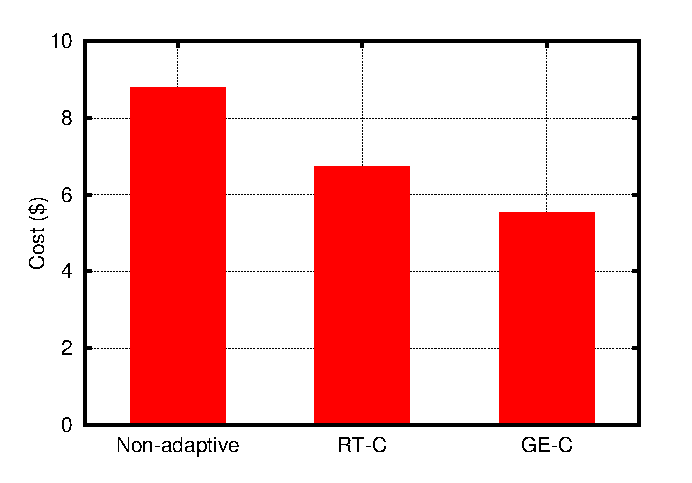
\includegraphics[scale=.7]{Graphs/cost.eps}
\caption{Cost analysis for VM usage}
\label{fig:cost}
\end{figure}

\section{Related Work}


%The increasing enthusiasm and consciousness of reducing energy consumption leads to smarter ways to consume energy in cloud data centers. While an efficient energy management technique in data center can reduce unnecessary use of brown energy and better utilize green energy without going to waste, smarter ways of consuming energy by an application can further reduce carbon footprint.


\paragraph*{\textbf{Green Energy aware Application adaptation}}

%rutgers work 2ta, yunbo work, geo distributed cloud.
%batch job
Goiri et al. \cite{GreenSlot} proposed \emph{GreenSlot}, a parallel batch job scheduler for a datacenter powered by an on-site renewable plant. Based on the historical data and weather forecast, GreenSlot predicts the amount of solar energy that will likely to be available in the future and subject to its predictions, it schedules the workload by the order of least slack time first (LSTF), to maximize the green energy consumption while meeting the job's deadlines by creating resource reservations into the future. Later, their work evolved into data processing framework by proposing \emph{GreenHadoop} \cite{GreenHadoop}. The idea relies on deferring background
computations \emph{e.g.,} data and log analysis, long simulations etc. that can be delayed by a bounded amount of time in a data center to take advantage of green energy availability while minimizing brown electricity cost. The idea is to run fewer servers when brown energy is cheap, and even fewer (if at all necessary) when brown energy is expensive. In conclusion, their proposal leads to operating few
hadoop clusters when green energy is scarce. 
Similar to this work, authors \cite{GreenPar} proposed \emph{GreenPar}, a scheduler for parallel high-performance applications to maximize using green energy in a partially powered data center and reduce brown energy consumption, while respecting performance aware SLA.  When green energy is available, GreenPar increases the resource allocations to active jobs to reduce runtimes by speeding up the processes while slow down the jobs to a maximum runtime slowdown percentage that is defined in SLA during the scarcity of the green energy. However, all these works focused specifically around batch like applications where job arrives with a deadline, hence can be deferred and scheduled by following the green energy availability. On the other hand, we propose to create green energy awareness around the interactive kind of application to to be self adapted with the presence/absence of green energy. Recently, Klein et al. \cite{brownout} introduced Brownout paradigm for dynamic adaptation in interactive application through control theory to withstand in
unpredictable runtime variations. Content reconfiguration takes into account only the system response time so that to prevent system instability in sudden workload burstiness. While the novelty of the approach is well understood,
how the controller should be designed to take the advantage of the presence of green energy and 
implemented in
massively virtualized and distributed cloud environment to exploit the elastic nature of infrastructure,
has not been addressed.

%geo-distributed cloud!
To this, in \cite{GreenWare}, the authors proposed \emph{GreenWare}, a middleware system that maximize the usage of green energy in geo-distributed cloud scale data centers by dynamically dispatching workload requests by following renewable, subject to energy budget constraint. The middleware performs three steps: computes the hourly energy budget and historical behavior of workload, runs an optimization algorithm based on constrained optimization technique, lastly dispatches requests according to optimization plan. Similar to this, \cite{not-easy} proposed a flow optimization based framework for request-routing considering the trade-off between access latency, carbon footprint and electricity costs to upgrade the plan of choosing data center in specific intervals. Again these works focused more on load-balancing of user requests to different data centers to maximize the usage of green energy rather relying on application adaptation on the fly.



\paragraph*{\textbf{Platform adaptation}}

%put corentin dupont's work here. Some other functional-Non functional adaptation.
Shi et al. \cite{shi} proposed two control layer, one responsible for allocating resources to VM's depending on the performance, the other one as a power saving layer to dynamically save energy by tuning voltage and frequency (DVFS) while resource requirement is low. Both layers are designed as autonomic loops in a coordinated
manner to control cluster level resources. Later, Hankendi et al. \cite{adaptcap} proposed an adaptive framework that jointly utilizes system (DVFS) and application-level
adaptation to improve efficiency of multi-core servers and reduction of power consumption. Application-level adaptation has been utilized to meet the performance
and accuracy constraints, whereas to meet power constraints, system-level
management was adopted. On the other hand, we propose to adopt sequential execution  of adaptation technique both at application and infrastructure level that not only met performance but also reduced energy consumption at significant portion. 

In contrast to prevoius works, authors at \cite{corentin} presented an Energy Adaptive Software Controller (\emph{EASC}) to make task and service oriented application adaptive to renewable energy availability. The work was part of by DC4Cities project \footnote{An European project on environmentally sustainable data centers for smart cities. Ended on 2016. \url{http://www.dc4cities.eu}}, which aimed at gathering renewable energy related information from energy providers and energy constraint directives from Energy monitoring authority (in context of Smart city) through an interface. Following the information, the PaaS layer is responsible to adapt the application by satisfying energy related constraints to consume more green energy, therefore building more eco-efficient policies for data center. The authors proposed to forward the energy related information to PaaS level via an API, so that an optimization plan can be invoked which involves desired working modes of an application considering energy and SLA constraints. However, service oriented application \emph{i.e.,} interactive application is defined as running web, database and mail servers and higher mode depicts multiple data center site is active with full capacity while lowest mode indicates running a single site with minimum capacity. Apart from that, Moreno et al. \cite{garlan1} proposed how different non-conflicting tactics (\emph{e.g.,} remove one software component and add one server) can be triggered simultaneously so that system can transition from current to desired state. The challenge is to estimate how two types of tactics when applied together reacts to the system. For instance, removing software component can have immediate transition, whereas adding one server can make a delayed transition which is also associated with cost. Depending on the goal, the utility function can be maximized by choosing proper adaptation tactics. Again these works ignored how to adapt and define tactics to leverage green energy availability to either consume more green energy or less brown energy.


\section{Conclusion}

In this article, we proposed a green energy aware platform that creates awareness around interactive Cloud application and formulate strategy to understand when to trigger scaling decision based on reactive and pro-active scaling rules. Secondly, we use traditional API such as \emph{scale-in} and \emph{scale-out} to trigger decision based on the strategy we have devised. Later we validated our approach by extensive experiments and results obtained over Grid'5000 test bed. Results showed that, significant amount of brown energy and cost reduction is possible if application can be adapted based on green energy availability.
For future work, we want to leverage micro-service architecture of an application to adapt itself in the presence of green energy. It would be interesting to deploy small and decoupled units of the application
throughout different containers (rather than VM) so that, each of the application component if required, can be scaled to guarantee better performance, self healing capabilities. Apart from that, resource can be assigned to specific components where it is required, thus over-provisioning of resource phenomena can be avoided resulting lesser energy consumption. Additionally, this investigation can leads to a decentralized autonomic behavior in modern
application. 



\bibliographystyle{ACM-Reference-Format}
\bibliography{bibliography} 

\end{document}
